\documentclass{article}

\usepackage{xeCJK}
% 段落缩进
\usepackage{indentfirst}
% 参考文献
\bibliographystyle{alpha}
% 链接参考文献和引用
\usepackage{hyperref}
% 索引
\usepackage{makeidx}
\makeindex
% 图片
\usepackage{graphicx}
% 标题
\usepackage{caption}
\captionsetup{figurename=图, tablename=表}
% 页面尺寸
\usepackage{geometry}
\geometry{a4paper, left=2cm, right=4cm, top=2cm, bottom=2cm}
% 程序代码
\usepackage{listings}
% 列表
\usepackage{enumitem}

\title{文章标题}
\author{周加根(zhoujiagen@gmail.com)}
%\date{2016-02-19}

% 在Mac应用>字体册.app中查看
%\setCJKmainfont{Lantinghei SC Extralight}
\setCJKmainfont[BoldFont={STHeiti}]{Lantinghei SC Extralight}
\begin{document}
% 段落间距
\setlength{\parskip}{0.5em}

\maketitle

\renewcommand\abstractname{简述}
\begin{abstract}
% 段落间距
\setlength{\parskip}{0.5em}
文章的简述
\end{abstract}

\newpage

\renewcommand\contentsname{目录}
\tableofcontents

\newpage

% 嵌入文档
%%%%%%%%%%%%%%%%%%%%%%%%%%%%%%%%%%%%%%%%%%%%%%%%%%%%%%%%%%%%
\section{Section 1}

Section 1 Content.

%% 列表
\begin{enumerate}[itemsep=0pt,parsep=0pt,label=(\arabic*)]
\item item1

item1 content.

\item item2

item2 content.

\end{enumerate}

\subsection{SubSection 1}

SubSection content.


% 代码字体
\texttt{int main() {}}

% 大段代码
\lstset{ basicstyle=\ttfamily, keywordstyle=\bfseries, commentstyle=\ttfamily, numbers=right, numberstyle=\footnotesize }
\begin{lstlisting}[language=C]
	#include <stdio.h>
	main() {
	    printlf("Hello world.\n");
	}
\end{lstlisting}

\newpage


%%%%%%%%%%%%%%%%%%%%%%%%%%%%%%%%%%%%%%%%%%%%%%%%%%%%%%%%%%%%
\section{Section 2}

% 索引
\index{HDFS}

% 文献引用
\cite{frontiers-mda}

% 交叉引用
%\ref{subsubsec:reservewords}(P.\pageref{subsubsec:reservewords})

% 图片和图片引用
HDFS中文件写入步骤见图\ref{fig:hdfs-write-data}:

\begin{figure}
\centering
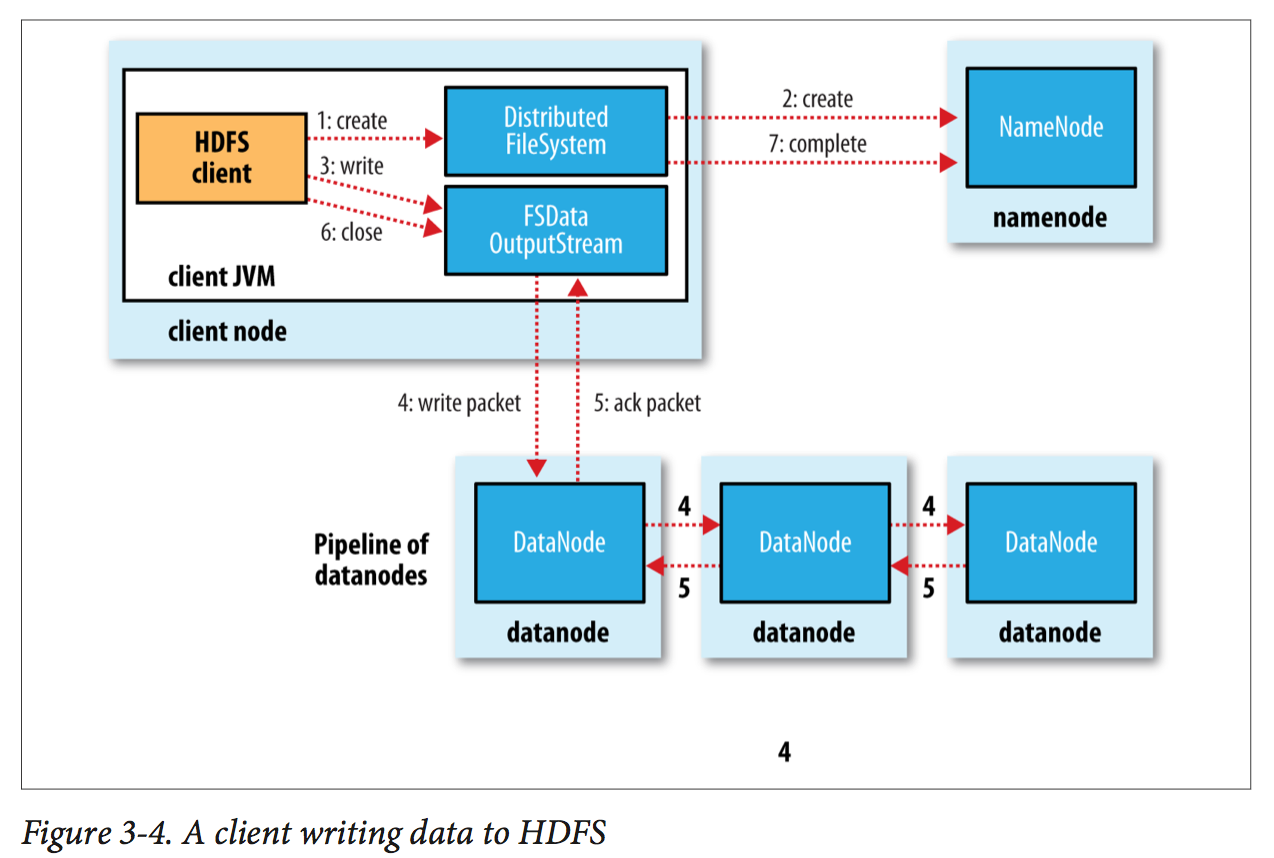
\includegraphics[scale=0.5]{image/hdfs-write-data.png}
\caption{HDFS数据写入}\label{fig:hdfs-write-data}
\end{figure}


\newpage
\renewcommand\refname{参考文献}
\bibliography{references}

\newpage
\renewcommand\indexname{索引}
\printindex

\end{document}
